\section{Another Conception of Triangles}\label{sect:streams}
In this section, we show another way to perceive and represent
infinite triangles. And we propose two ways of defining redecoration
on this new representation. 

\subsection{A new definition using streams}
In the previous section, we always visualized the infinite triangles
by their columns. Indeed, we said that a triangle was a first column
with only one element of type $A$ (the element of the diagonal) and a
trapezium, itself actually a triangle, as suggested in
\rfig{visu_col}. 

While elements of the finite triangles in $\Trif\,A$ (see
\rsect{intro}) are (globally) finite, also all the columns of our
infinite triangles in $\Tri\,A$ are finite. In the work that we
started from for this article \cite{types07},
redecoration on $\Trif$ is verified against a model where triangles
are represented by finite lists of columns, where each column consists
of the diagonal element in $A$ and a finite list of elements in $E$. A
naive dualization of that approach would consist in taking as
representation of infinite triangles streams of columns that would be
formed as for the finite ones. This mixture of inductive and
coinductive datatypes is notoriously difficult to handle. We have been
confronted with this problem many times in the last few years, as can
be seen in the second author's thesis \cite{theseCP} which deals with this kind of problems
particularly in Coq. But in other proof assistants, the same kind of
issues has appeared; there is also an experimental solution in Agda \cite{dan, daal}.  Still, the representation of infinite
triangles mixing inductive and coinductive datatypes can be carried
out, but we refrain from presenting this column-based approach here.

However, we can also visualize triangles the other way around. We now consider
the triangle by its rows, as suggested in \rfig{visu_row}.  
\begin{figure}[h]
  \centering
  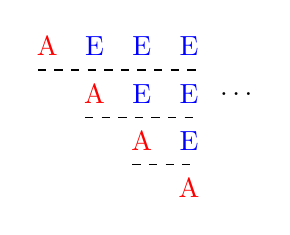
\begin{tikzpicture}[scale = 0.6]
    \foreach \y in {0,...,2}
    {\foreach \x in {\y,...,2}
      \draw (\x+1, -\y) node[color=blue]{E} ;
    }
    \foreach \x in {0,...,3} \draw (\x, -\x) node[color=red]{A} ;
    \draw(4,-1) node{$\ldots$};
    \draw[style = dashed](-0.2,-0.5) -- (3.2,-0.5);
    \draw[style = dashed](0.8,-1.5) -- (3.2,-1.5);
    \draw[style = dashed](1.8,-2.5) -- (3.2,-2.5);
  \end{tikzpicture}
  \vspace{-3ex}
  \caption{Dividing a triangle into rows}
  \label{fig:visu_row}
\end{figure}
Then, on any row, we have one element of type $A$ and infinitely many
elements of type $E$. And we also have infinitely many rows. Here,
nothing is finite (only the single element of $A$ at the head of each
row, but this is not a problem), therefore, we do not have any
embedded inductive type in our description -- unlike in the columnwise
decomposition mentioned above. This new visualization can be
represented as a stream of pairs made of one element of type $A$ and a
stream of elements of type $E$.

\begin{definition}
  $\TriS\,A := \Str (A \times \Str\,E)$
\end{definition}
Actually, following the definition of \Str{}, we can read this new definition of the triangles as
consisting of three parts: the top element, the stream of elements of
$E$ of the first row and the triangle corresponding to the rest, as
shown in \rfig{3elems}.
\begin{figure}[h]
  \centering
  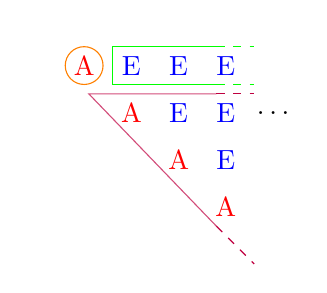
\begin{tikzpicture}[scale = 0.6]
    \foreach \y in {0,...,2}
    {\foreach \x in {\y,...,2}
      \draw (\x+1, -\y) node[color=blue]{E} ;
    }
    \foreach \x in {0,...,3} \draw (\x, -\x) node[color=red]{A} ;
    \draw(4,-1) node{$\ldots$};
    \draw[color=orange] (0,0) circle(0.4cm);
    \draw[color=orange] (-1,0) node{$\topS$};

    \draw[color=green] (2.8,0.4) -- node[auto, swap, above]{\frowS} (0.6,0.4) --
    (0.6,-0.4) -- (2.8,-0.4);
    \draw[color=purple!70]  (2.8,-0.6) --  (0.1,-0.6) -- node[auto, swap,
    left]{\restS}(2.8, -3.4);
     \draw[color=green, style = dashed](2.8,0.4) -- (3.6,0.4);
     \draw[color=green, style = dashed](2.8,-0.4) -- (3.6,-0.4);
     \draw[color=purple, style = dashed](2.8,-0.6) -- (3.6,-0.6);
     \draw[color=purple, style = dashed](2.8,-3.4) -- (3.6,-4.2);
  \end{tikzpicture}
  \vspace{-3ex}
  \caption{Conceptualizing a triangle as a triple}
  \label{fig:3elems}
\end{figure}

\noindent
We define functions that allow us to access to each of these elements: 
\begin{definition}[Projections]\ 
  $$
  \begin{array}{l@{\hspace{2em}}l@{\hspace{2em}}l}
    \topS : \forall A.\,\TriS\,A \to A &
    \frowS : \forall A.\, \TriS\,A \to \Str\,E &
    \restS: \forall A.\, \TriS\,A \to \TriS\,A \\
    \topS\,(\pair{a}{\es} :: t) := a&
    \frowS\,(\pair{a}{\es} :: t) := \es&
    \restS\,(\pair{a}{\es} :: t) := t
  \end{array}
  $$
\end{definition}
Notice that $\rest$ and $\restS$ are conceptually different -- the
former yields the trapeziums after cutting off the first column, the
latter triangles after cutting off the first row.

To compare two elements of \TriS{}, we need a notion of bisimilarity, which on \Str{} is pre-defined in
Coq as follows:
\begin{definition}[$\EqSt:\forall C.\,\Rel(\Str\,C)$, defined
  coinductively]\ 
        \begin{prooftree}
          \AxiomC {$s_1\,,\, s_2 : \Str\,C$}
          \AxiomC {$\hd\,s_1 = \hd\,s_2$}
          \AxiomC {$\tl\,s_1\EqSt\tl\,s_2$}
          \doubleLine
          \TrinaryInfC{$s_1\,\EqSt\, s_2$}
        \end{prooftree}
\end{definition}

However, we cannot use it directly. Indeed, we would need to prove,
for two triangles $t_1$ and $t_2$ that their first rows are
Leibniz-equal, i.\,e., $\frowS\,t_1 = \frowS\,t_2$. This is too
strict, since the rows are defined partially coinductively (because of
the stream of $E$'s). Therefore, we need to define a new relation on
\TriS{} that will compare the three elements of the triangles. The
tops can be compared through Leibniz equality, the first rows can be
compared using \EqSt{} and the rests with the relation on \TriS,
corecursively.
\begin{definition}[$\bisimS:\forall A.\,\Rel(\TriS\,A)$, defined
  coinductively]\label{lemma:bisimS}\ 
  \begin{prooftree}
    \AxiomC {$t_1\,,\, t_2 : \TriS\,A \hspace{5ex} \topS\,t_1 = \topS\,t_2$}
    \AxiomC {$\frowS\,t_1\EqSt\frowS\,t_2$}
    \AxiomC {$\restS\,t_1 \bisimS \restS\,t_2$}
    \doubleLine
    \TrinaryInfC{$t_1\,\bisimS\, t_2$}
  \end{prooftree}
\end{definition}
It is immediate to show that \bisimS{} is an equivalence relation. 

In order to validate this view of the triangles, we want to show that
it is indeed equivalent to the original one. Therefore, we are going
to show that there is a bijection between the two definitions (modulo
pointwise bisimilarity). To do so we define two conversion functions
(\tSR{}, from \Tri{} to \TriS{} and \fSR{} for the other way around) and show that their
compositions are pointwise bisimilar to the identity.

The two conversion functions are quite natural. To transform an
element of $\Tri\,A$ into an element of $\TriS\,A$, we need to reconstruct from
the original triangle the three elements of $\TriS\,A$. The top remains
the original top, this is trivial. The first row of elements of $E$ is given by \frow. Finally,
the triangle has to be transformed again by \tSR{} from the rest of
the triangle with the first row cut out by the function \cut. The
calculation for the different parts is represented in \rfig{tSR}. 
\begin{figure}[h]
  \centering
  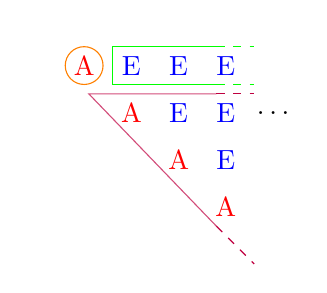
\begin{tikzpicture}[scale = 0.6]
    \foreach \y in {0,...,2}
    {\foreach \x in {\y,...,2}
      \draw (\x+1, -\y) node[color=blue]{E} ;
    }
    \foreach \x in {0,...,3} \draw (\x, -\x) node[color=red]{A} ;
    \draw(4,-1) node{$\ldots$};
    \draw[color=orange] (0,0) circle(0.4cm);
    \draw[color=orange] (-1,0) node{$\topT$};

    \draw[color=green] (2.8,0.4) -- node[auto, swap, above]{\frow} (0.6,0.4) --
    (0.6,-0.4) -- (2.8,-0.4);
    \draw[color=purple!70]  (2.8,-0.6) --  (0.1,-0.6) -- node[auto, swap,
    left]{\cut~\rest}(2.8, -3.4);
     \draw[color=green, style = dashed](2.8,0.4) -- (3.6,0.4);
     \draw[color=green, style = dashed](2.8,-0.4) -- (3.6,-0.4);
     \draw[color=purple, style = dashed](2.8,-0.6) -- (3.6,-0.6);
     \draw[color=purple, style = dashed](2.8,-3.4) -- (3.6,-4.2);
  \end{tikzpicture}
  \vspace{-3ex}
  \caption{Definition of \tSR}
  \label{fig:tSR}
\end{figure}
\begin{definition}[$\tSR: \forall A.\, \Tri\,A \to \TriS\,A$, defined corecursively]\label{def:tSR}
  $$\tSR\,t := \pair{\topT\,t}{\frow\,t} :: \tSR \,(\cut\, (\rest\,t))$$
\end{definition}
The definition of \fSR{} is also quite intuitive. We have to construct
the two elements that compose elements of type \Tri{}. The top remains
the top as before, this is again trivial. For the rest, we have to ``glue''
the first row to the rest of the triangle (basically the inverse of
the \cut{} and \escut{} functions on \TriS) before transforming it
again. 
We call \addesS{} the function that performs this operation, as shown
in \rfig{addesS}. 
\begin{figure}[h]
  \centering
  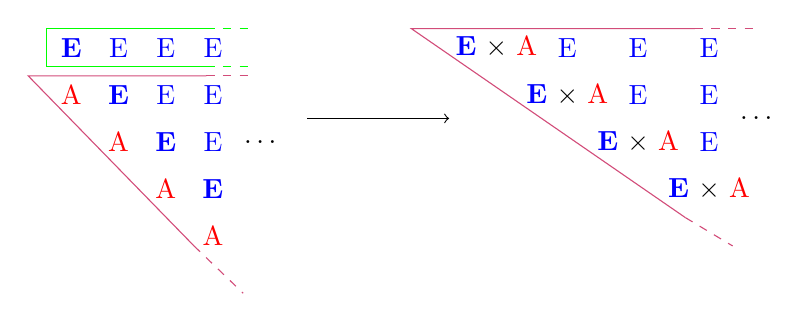
\begin{tikzpicture}[scale = 0.6]

    \foreach \y in {0,...,2}
    {\foreach \x in {\y,...,2}
      \draw (\x+1, -\y) node[color=blue]{E} ;
    }
    \foreach \x in {0,...,3} \draw (\x, -\x-1) node[color=red]{A} ;
    \foreach \x in {0,...,3} \draw (\x, -\x)
    node[color=blue]{\textbf{E}} ;
    \draw(4,-2) node{$\ldots$};

    \foreach \y in {0,...,2}
    {\foreach \x in {\y,...,2}
      \draw (1.5*\x+10.5, -\y) node[color=blue]{E} ;
    }
    \foreach \x in {0,...,3} \draw (1.5*\x+9, -\x)
    node{{\color{blue}\textbf{E}} $\times$ {\color{red} A}} ;
    \draw(14.5,-1.5) node{$\ldots$};
    
    \draw[->] (5,-1.5) to node[swap, auto, above]{\addesS}
    (8,-1.5) ; 

     \draw[color=green] (2.2*1.3,0.4) -- (-0.4*1.3,0.4) -- 
     (-0.4*1.3,-0.4) -- (2.2*1.3,-0.4);
     \draw[color=purple!70] (2.2*1.3,-0.6) -- (-0.7*1.3,-0.6) --
     (2*1.3, -4.2) ; 
     \draw[color=green, dashed] (2.2*1.3,0.4) -- (3*1.3,0.4);
     \draw[color=green, dashed] (2.2*1.3,-0.4) -- (3*1.3,-0.4);
     \draw[color=purple!70, dashed] (2.2*1.3,-0.6) -- (3*1.3,-0.6);
     \draw[color=purple!70, dashed] (2*1.3,-4.2) -- (2.8*1.3,-5.2);

     \draw[color=purple!70] (13.2,0.4) -- (7.2,0.4) -- (13, -3.6); 
     \draw[color=purple!70, dashed] (13.2,0.4) -- (14.5,0.4);
     \draw[color=purple!70, dashed] (13,-3.6) -- (14,-4.2);
    
  \end{tikzpicture}
  \caption{Definition of \addesS}
  \label{fig:addesS}
\end{figure}
\begin{definition}[$\addesS: \forall A.\, \Str\,E \to \TriS\,A \to \TriS
  (E\times A)$, defined corecursively]\label{def:addesS}
  $$\addesS\,(e :: \es)\,t := \pair{\pair{e}{\topS\,t}}{\es} :: \addesS\,(\frowS\,t)\,(\restS\,t)$$
\end{definition}
\begin{definition}[$\fSR: \forall A.\, \TriS\,A \to \Tri\,A$, defined corecursively]\label{def:fSR}
  $$\fSR\,t := \constr\,(\topS\,t)\,\bigl(\fSR\,(\addesS\,(\frowS\,t)\,(\restS\,t))\bigr)$$
\end{definition}
\begin{remark}
  Our first idea was to do the gluing after the
  transformation. Indeed, as the transformation does not affect the
  elements of $E$, it seemed more natural to us not to submit this
  part to the corecursive call of the transformation.
  Thus, we wanted to define \fSR{} coinductively as follows:
  $$ \fSR\,t := \constr\,(\topS\,t)\,(\addes\,(\frowS\,t)\,(\fSR\,
  (\restS\,t)))$$
  However, even if this seems harmless, this definition cannot be
  accepted by Coq since the corecursive call to \fSR{} is not
  guarded (it is an argument of \addes{} and not of a constructor). Nevertheless, we have shown that the solution to the
  previous equation is unique with respect to pointwise bisimilarity and that
  \fSR{} of \rdef{fSR} satisfies it. 
\end{remark}
\begin{lemma}\label{lemma:tSR_fSR}
  $\forall A\forall(t:\TriS\,A).\, \tSR\, (\fSR\,t) \bisimS t$
\end{lemma}
\begin{proof}
  To prove this result, we actually prove the following stronger
  result that we then only instantiate to finish the proof: 
  $$\forall A\forall (t:\TriS\,A)(u:\Tri\,A),\, \tSR \,(\fSR\,t) \bisimS u \Rightarrow t \bisimS u $$
  The proof of this statement is a simple coinduction, that uses some
  straightforward results on \cut{} and \addesS{}. 
\end{proof}
\begin{lemma}\label{lemma:fSR_tSR}
  $\forall A\forall (t:\Tri\,A).\, \fSR\, (\tSR\,t) \bisim t$
\end{lemma}
\begin{proof}
  We use the same technique as before. We prove a stronger result that
  we instiantiate to prove our lemma: 
  $$\forall A\forall (t:\Tri\,A)(u:\TriS\,A).\, \fSR\, (\tSR\,t) \bisim u \Rightarrow t \bisim u $$
  Here again, the proof is a straightforward coinduction using
  compatibility of \topT{} and \rest{} with $\bisim$ and a simple result on \addesS.
\end{proof}

\subsection{Redecoration on \TriS{}}
Thus, we have a completely different view of the triangles, but still,
it is fully equivalent to the original one.  The interest of this view
is that now the redecoration is very easy to perform. Indeed, before,
the tricky part was that we had to lift the function $f$ to
trapeziums, and therefore to cut out the elements of $E$ remaining
(implicitly) from the first row. The problem was that we roughly had to
cut out a row, while we were reasoning on columns. Here, as we
directly reason on rows, it is much easier. As shown in \rfig{redecS},
the three elements of the transformed triangle will be:
\begin{itemize}
  \item the top is the application of $f$ to the whole triangle (as before)
  \item the first row of elements of $E$ is  the same row as in the original
    triangle (and as we said we have direct access to it)
  \item the rest of the triangle is the application of the redecoration
    function to the rest
\end{itemize}

\begin{figure}[h]
  \centering
  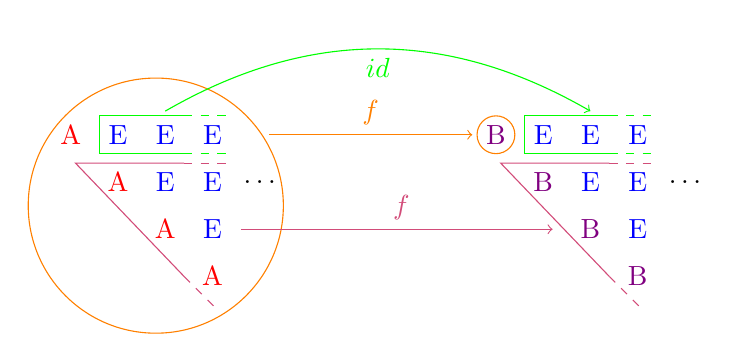
\begin{tikzpicture}[scale = 0.6]
    
    \foreach \y in {0,...,2}
    {\foreach \x in {\y,...,2}
      \draw (\x+1, -\y) node[color=blue]{E} ;
    }
    \foreach \x in {0,...,3} \draw (\x, -\x) node[color=red]{A} ;
    \draw(4,-1) node{$\ldots$};

    \foreach \y in {0,...,2}
    {\foreach \x in {\y,...,2}
      \draw (\x+10, -\y) node[color=blue]{E} ;
    }
    \foreach \x in {0,...,3} \draw (\x+9, -\x) node[color=violet]{B} ;
    \draw(13,-1) node{$\ldots$};
    \draw[color=purple!70]  (2.4, -3) --
    (0.1,-0.6) --  (2.4,-0.6);
    \draw[color=purple!70, dashed]  (2.4,-0.6) -- (3.4,-0.6);
    \draw[color=purple!70, dashed]  (2.4,-3) -- (3.1,-3.7);
 
    \draw[color=orange] (1.8,-1.5) circle(2.7cm);

    \draw[color=purple!70]  (11.4, -3) --
    (9.1,-0.6)-- (11.4,-0.6);
    \draw[color=purple!70, dashed]  (11.4,-0.6) -- (12.4,-0.6);
    \draw[color=purple!70, dashed]  (11.4,-3) -- (12.1,-3.7);
    
    \draw[color=orange] (9,0) circle(0.4cm);
    
    \draw[->,color = orange] (4.2,0) to node[auto,
    swap, above]{$f$} (8.5,0) ; 

    \draw[->,color = purple!70] (3.6,-2) to  node[auto,
    swap, above]{$\redecS~f$} (10.2,-2) ;
    \draw[->,color = green] (2,0.5) to [bend left] node[auto,
    swap, below]{$id$} (11,0.5) ;  


    \draw[color=green] (2.4,0.4) --  (0.6,0.4) -- 
    (0.6,-0.4) -- (2.4,-0.4);
    \draw[color=green, dashed]  (2.4,0.4) -- (3.4,0.4);
    \draw[color=green, dashed]  (2.4,-0.4) -- (3.4,-0.4);

    \draw[color=green] (11.4,0.4) --  (9.6,0.4) -- 
    (9.6,-0.4) -- (11.4,-0.4);
    \draw[color=green, dashed]  (11.4,0.4) -- (12.4,0.4);
    \draw[color=green, dashed]  (11.4,-0.4) -- (12.4,-0.4);

  \end{tikzpicture}
  \caption{Definition of redecoration}
  \label{fig:redecS}
\end{figure}

\noindent
Therefore, we can define the redecoration function for \TriS{} as
follows: 
\begin{definition}[$\redecS: \forall A\forall B.\,(\TriS\,A\to B)\to \TriS\,A\to\TriS\,B$, defined corecursively]\label{def:redecS}
  $$\redecS\,f\,t := \pair{f\,t}{\frowS\,t} :: \redecS\,f\,(\restS\,t)$$
\end{definition}
We can finally show that this new version of the redecoration is
equivalent to the previous one, modulo compatibility, using the conversion functions. We
show that:
\begin{lemma}\label{lemma:redecS_redec}
  $$
  \begin{array}{rl}
    \forall f, &
    (\forall t\,t', t \bisimS t' \Rightarrow f\,t = f\,t') \\
    \Rightarrow &
    \forall t, \redecS\,f\,t \bisimS \tSR\,(\redec\,(f \circ
    \tSR)\,(\fSR\,t)) 
  \end{array}
  $$ 
\end{lemma}
\begin{lemma}\label{lemma:redec_redecS}
  $$
  \begin{array}{rl}
    \forall f, &
    (\forall t\,t', t \bisim t' \Rightarrow f\,t = f\,t') \\
    \Rightarrow & \forall t, \redec\,f\,t \bisim \fSR\,(\redecS\,(f \circ
    \fSR)\,(\tSR\,t)) 
  \end{array}
  $$
\end{lemma}
\begin{remark}
  The compatibility hypotheses here are needed to work with \Tri{}. Up
  to these extra requirements, the two conversion functions yield an
  isomorphism of comonads (the associated properties for \topT{} and
  \topS{} are immediate by definition).
\end{remark}


\subsection{Simplifying redecoration again}

As the representation of infinite triangles \TriS{} is only as a stream
of streams, we can use standard functions on streams to define
redecoration. Indeed, redecoration can be interpreted as
consisting of applying a function to each element of the diagonal of
an infinite triangle, where each element of the diagonal is itself a
triangle (iterated tails of the given triangle). We can thus decompose the
redecoration operation into two steps: first transform the infinite
triangle into a triangle of triangles and then apply the
transformation function on the elements of the diagonal, as shown in
\rfig{redecS'_id}.
\begin{figure}[h]
  \centering
  \begin{tikzpicture}[scale = 0.6]
    
    \foreach \y in {0,...,2}
    {\foreach \x in {\y,...,2}
      \draw (\x+1, -\y-2) node[color=blue]{E} ;
    }
    \foreach \x in {0,...,3} \draw (\x, -\x-2) node[color=red]{A} ;
    \draw(4,-3) node{$\ldots$};


    \foreach \y in {0,...,2}
    {\foreach \x in {\y,...,2}
      \draw (1.7*\x+9.5, -2*\y-1) node[color=blue]{E} ;
    }
    
    
    \foreach \x in {0,...,2} 
    {
      
      \foreach \b in {0,...,\x}
      {\foreach \a in {0,...,\b}
        \draw (7.5+\b*0.5+4-\x*2, -\a*0.5-4+\x*2) node[color=orange,scale=0.6]{E} ;
      }
      \foreach \a in {\x,...,3} \draw (1.5*\x+7+\a*0.5, -\a*0.5-\x*1.5) node[color=orange,scale=0.6]{A} ;
      \draw(1.5*2-1.5*\x+9,-4.3+\x*1.8) node[color=orange, scale=0.5]{$\ldots$};
      
    }
    \draw (12.8,-6) node[color=orange, scale=0.6]{A};
    \draw (13.2,-6) node[color=orange, scale=0.5]{$\ldots$};
    \draw(14,-3) node{$\ldots$};

    \foreach \y in {0,...,2}
    {\foreach \x in {\y,...,2}
      \draw (\x+19, -\y-2) node[color=blue]{E} ;
    }
    \foreach \x in {0,...,3} \draw (\x+18, -\x-2) node[color=violet]{B} ;
    \draw(22,-3) node{$\ldots$};

    \draw[->,color = purple!80] (4.8,-3) to node[auto,
    swap, below]{$1^{\textrm{st}}$ step} (8.5,-3) ; 
    \draw[->,color = purple!80] (14.8,-3) to node[auto,
    swap, below]{$2^{\textrm{nd}}$ step} (18.5,-3) ; 

  \end{tikzpicture}
  \vspace{-1ex}
  \caption{Idea of another definition of redecoration}
  \label{fig:redecS'_id}
\end{figure}

\begin{remark}
  \rfig{redecS'_id} is only a visualization of what happens, and has
  to be taken lightly. In particular, all the elements of the diagonal
  of the middle triangle are infinite triangles, as we said. But, in
  order to visualize better what we do, their size seems to decrease
  since we cut out the first row of the previous element of the
  diagonal. 
\end{remark}
\noindent
These two steps are then trivial to define on streams. Indeed, the
first step consists of replacing all the elements of $A$ by the
corresponding iterated tail of the triangle itself. In fact, the
information about the elements of $E$ is redundant. Indeed, it is
contained in the terms of the diagonal themselves (the row of elements
of $E$ ``to the right'' of an element of the diagonal is the first row
of this element, minus the element of $A$). Therefore, we can omit
them and only concentrate on the triangles. Thus, we need to obtain
the stream of all the iterated tails of the initial triangle (see the
first part of \rfig{redecS'}). This is given by the classical \tls{}
operation defined below:
\begin{definition}[$\tls:\forall C.\,\Str\,C\to\Str(\Str\,C)$, viewed coinductively]
  $\tls\,s := s :: \tls (\tl\,s)$
\end{definition}
\begin{remark}
  The function \tls{} has the signature of the comultiplication
  operation in a comonad based on \Str{} according to the classical
  definition of comonads \cite{maclane} (the term
  ``comultiplication'' is not used there, but only the letter $\delta$
  that is dual to the multiplication of a monad). See
  \rlem{StrComonad} below for the constructive comonad based on
  \Str{}.
\end{remark}
\noindent
In \rfig{redecS'_id}, the second step only consists of applying $f$ to
all the elements of the diagonal. In fact, the first step corresponds
to transforming $t$ of type $\TriS\,A$ into
$$\map\,\bigl(\lambda x.\pair x{\frowS\,x}\bigr)\,(\tls\,t)\enspace,$$
and the second one consists in transforming $s$ of type $\TriS(\TriS\,A)$ into
$$\map\,\bigl(\lambda\pair u\es.\,\pair{f\,u}\es\bigr)\,s\enspace.$$

We can alternatively see the transformation of $t$ into $\tls\,t$ as
the first step, and the two successive $\map$ operations as the second
step, which is therefore (by applying the functor law for $\map$
saying that $\map$'s compose) performed by $\map\,(\liftS\,f)$, with
$\liftS$ defined as follows:
\begin{definition}[$\liftS: \forall A\forall B.\,(\TriS\,A\to B)\to \TriS\,A\to B\times\Str\,E$]
$$\liftS\,f:=\lambda x.\pair{f~x}{\frowS~x}$$
\end{definition}
As for \rest{} and \restS{}, \lift{} and \liftS{} are unrelated and
belong to the respective point of view.  This new version of the
redecoration operation is shown in \rfig{redecS'}.
\begin{figure}[h]
  \centering
  \begin{tikzpicture}[scale = 0.6]
    
    \foreach \y in {0,...,2}
    {\foreach \x in {\y,...,2}
      \draw (\x+1, -\y) node[color=blue]{E} ;
    }
    \foreach \x in {0,...,3} \draw (\x, -\x) node[color=red]{A} ;
    \draw(4,-1) node{$\ldots$};

    \draw (6, -0.7) node{$\Bigg [$} ;
    \draw (16, -0.7) node{$\Bigg ]$} ;
    
    \foreach \x in {0,...,2} 
    {
      
      \foreach \b in {0,...,\x}
      {\foreach \a in {0,...,\b}
        \draw (2*2.8-2.8*\x+7.3+\b*0.5, -\a*0.5-1+\x*0.5) node[color=orange,scale=0.6]{E} ;
      }
      \foreach \a in {\x,...,3} {
        \draw (2.3*\x+6.8+\a*0.5, -\a*0.5) node[color=orange,scale=0.6]{A} ;
      }
      \draw(2.3*\x+8.7,-0.5-\x*0.4) node[color=orange,
      scale=0.5]{$\ldots$};
      \draw(2.3*\x+9.2,-0.7) node{;};
    }
    \draw(14.2,-1.5) node[color=orange, scale=0.6]{A};
    \draw(14.7,-1.5) node[color=orange, scale=0.5]{$\ldots$};
    \draw(15,-0.7) node{;};
    \draw(15.5,-0.7) node{$\ldots$};

    \foreach \y in {0,...,2}
    {\foreach \x in {\y,...,2}
      \draw (\x+19, -\y) node[color=blue]{E} ;
    }
    \foreach \x in {0,...,3} \draw (\x+18, -\x) node[color=violet]{B} ;
    \draw(22,-1) node{$\ldots$};

    \draw[->,color = purple!80] (2,0.5) to [bend left] node[auto,
    swap, above]{$\tls$} (10,0.5) ; 
    \draw[->,color = purple!80] (11,0.5) to [bend left] node[auto,
    swap, above]{$\map~(\liftS\,f)$} (19,0.5) ; 

  \end{tikzpicture}
  \caption{Another definition of redecoration}
  \label{fig:redecS'}
\end{figure}

Thus, we define a new version of the redecoration operation as
follows:
\begin{definition}[$\redecSS : \forall A\forall B.\,(\TriS\,A \to B) \to
  \TriS\,A \to \TriS\,B$]
  $$\redecSS\,f\,t := \map\,(\liftS\,f)\,(\tls\,t)$$
\end{definition}
\noindent
One can then easily show that this operation is equivalent to the
previous one: 
\begin{lemma}
  $\forall A\forall B\forall (f: \TriS\,A \to B)\forall (t:
  \TriS\,A).\, \redecS\,f\,t \EqSt \redecSS\,f\,t$
\end{lemma}
The proof is a straightforward coinduction. 

It is interesting to note that here, we do not need the bisimulation
relation defined on \TriS{}. We can directly use the standard relation
on \Str{}, \EqSt{}. This should not be surprising. Indeed, here we
only really manipulate streams. Those streams are made of pairs and we
only manipulate the finite part of each pair (the first element). The
second one is only a copy. Therefore the relation \bisimS{} would be
artificial here. 

Let's continue abstracting and define \redecSG{} as follows:
\begin{definition}[$\redecSG: \forall A\forall B.\,(\Str\,A \to B) \to
  \Str\,A \to \Str\,B$]
  $$\redecSG\,f\,s :=  \map\,f\,(\tls\,s)$$
\end{definition}
\noindent
As we remarked previously, \tls{} has the signature of a
comultiplication for a comonad (in the triple format \cite{maclane}) based on \Str{},
and it is well known that \map{} is the functor (on morphisms) for
\Str{}. Therefore, \redecSG{} becomes the cobind operation of this
comonad, generically. We do not develop this piece of constructive
category theory here, but only state the result for this instance:
\begin{lemma}\label{lemma:StrComonad}
  The type transformation \Str{}, the projection function \hd{} and
  \redecSG{} form a constructive comonad with respect to \EqSt{}.
\end{lemma}

This section is inspired by Adriano
\cite{haskellList:redecorationAnswer}
who suggested 
a redecoration function for Haskell lists just
in this form. More precisely, a function \texttt{slide :: ([a] -> b) -> [a] ->
  [b]} was defined by \texttt{slide f = map f.tails}. Note that Haskell
lists can be finite and infinite, thus this definition captured
streams as well.

The function \redecSS{} is an instance of \redecSG{}, i.\,e.,
the following lemma is trivial: 
\begin{lemma}
  $\forall A\forall B\forall(f:\TriS\,A\to B)(t:\TriS\,A).\, \redecSS\,f\,t = \redecSG\,(\liftS\,f)\,t$
\end{lemma}
\noindent
Therefore, it is natural to show the three laws of comonads for
\redecSS{} and the proofs are much simplified by the use of
\redecSG{}. In particular, we can show a kind of commutativity of $\liftS$ with
\redecSS{}. 

\begin{lemma}
  The type transformation \TriS{}, the projection function \topS{}
  and \redecSS{} form a constructive comonad with respect to \EqSt{}
  (more precisely, the equivalence relation is
  $\EqSt_{A\times\Str\,E}$ for every $A$).
\end{lemma}
\begin{remark}
  Through the functions \tSR{} and \fSR{}, one can then transfer this
  comonad structure back to \Tri{}.  Since \rlem{redecS_redec} and
  \rlem{redec_redecS} require compatibility of $f$ with bisimilarity,
  this will not even give a constructive weak comonad, but the first
  and third law have to be relativized to compatible $f$'s as
  well. Still, this does not seem a problematic constraint. Anyway,
  \rlem{TriWComonad} has been proved independently of streams.
\end{remark}


%%% Local Variables:
%%% mode: latex
%%% TeX-master: "coredec"
%%% End:
